\documentclass[twocolumn,prb,showpacs,superscriptaddress]{revtex4}
\usepackage{graphicx}

%
% warning: if you redefine \r you will have troubles with the angstrom,
% which is internally defined as \r{A}
%

\def\w{\omega}
\def\>{\rangle}
\def\<{\langle}
\def\H{\hat{H}}
\def\P{\hat{P}_{\rm occ}}
\def\E{\varepsilon}
\def\vp{{v^\prime}}
\def\q{{\bf q}}
\def\s{\sigma}
\def\k{{\bf k}}
\def\qp{{\bf q^\prime}}
\def\G{{\bf G}}
\def\Gp{{\bf G^\prime}}
\def\rt{\tilde{r}}
\def\pt{\tilde{p}}
\def\r{{\bf r}}
\def\rp{{\bf r^\prime}}
\def\rpp{{\bf r^{\prime\prime}}}
\def\rppp{{\bf r^{\prime\prime\prime}}}

% -------
\usepackage{soul}
\usepackage{color}
\definecolor{yellow}{rgb}{1,1,0}
\definecolor{lightblue}{rgb}{0.6,0.6,0.9}
\sethlcolor{yellow}
% -------

\begin{document}

\title{GW method using density-functional perturbation theory}

\author{Feliciano Giustino}
\email{feliciano.giustino@materials.ox.ac.uk}
\affiliation{Department of Materials, University of Oxford, Parks Road, Oxford OX1 3PH, United Kingdom}
\affiliation{Department of Physics, University of California at Berkeley, 
Berkeley, California 94720, USA,
and Materials Sciences Division, Lawrence Berkeley National Laboratory, 
Berkeley, California 94720, USA}
\author{Marvin L. Cohen}
\author{Steven G. Louie}
\affiliation{Department of Physics, University of California at Berkeley, 
Berkeley, California 94720, USA,
and Materials Sciences Division, Lawrence Berkeley National Laboratory, 
Berkeley, California 94720, USA}
\date{\today}

\begin{abstract}
We propose a new approach to quasiparticle GW calculations based on the
direct evaluation of the Green's function and of the screened Coulomb interaction.
The Green's function is computed by using Haydock's recursion method,
and the screened Coulomb interaction is computed by using density-functional
perturbation theory. The frequency-dependent screened Coulomb interaction 
is explicitely calculated along the imaginary axis and analytically continued 
to the real axis using Pad\'e functions. We implemented the
proposed method within the empirical pseudopotential formalism and 
we studied silicon as a test case. We compare our new method with existing
approaches and illustrate our future development plans.
\end{abstract}

\pacs{71.15.-m, % Methods of electronic structure calculations
      71.15.Qe} % Excited states: methodology

\maketitle

\section{Introduction}

Importance of GW calculations, Motivation, History of the idea,
Explanation of where we are and how the manuscript is organized.

Must cite work of HL-dielectric where they discuss the direct approach
and find it problematic because of the supercell required.
Must cite Fleszar-Resta and Reining - they calculate epsilon.
Kunc-Tosatti calculate inveps but they do finite differences
(calculations with the KS potential + perturbation).

Our novelty is that we do self-consistency by using DFPT
and generalize DFPT to finite frequency calculations.

\section{Overview of the methodology}

\section{Screened Coulomb interaction}

We assume insulators with a finite gap. Generalization to the case of metals
can be done following De Gironcoli.
In the following we assume Rydberg atomic units (hence the Coulomb potential
will be $e^2/r$ with $e^2=2$ and $1/(4\pi\epsilon_0)=1$, and the kinetic energy $-\nabla^2$, since $\hbar=1$ 
and $2m_{\rm e}=1$).
The screened Coulomb interaction $W(\r,\rp;\w)$ can be calculated by using
the second one of Hedin's equations in space-frequency representation
[Eq.\ (13.19b) of Ref.~\onlinecite{hl}]:
  \begin{eqnarray}\label{eq.w}
  W(\r,\rp;\w) & = & v(\r,\rp) + \int d\rpp \,W(\r,\rpp;\w)  \nonumber \\
   & \times & \int d\rppp P(\rpp,\rppp;\w) v(\rppp,\rp), 
  \end{eqnarray}
$v(\r,\rp)=|\r-\rp|^{-1}$ being the bare Coulomb interaction (in Hartree units) and
$P(\r,\rp;\w)$ the irreducible polarization propagator. 
Within the random phase approximation the polarization propagator reads 
[Eq.\ (14.8) of Ref.~\onlinecite{hl}]:
  \begin{equation}\label{eq.p}
  P(\r,\rp;\w) = \sum_{n,m} \frac{f_n-f_m}{\E_n-\E_m-\w} 
  \psi_n(\r)\psi_m^\star(\r)  \psi_n^\star(\rp)\psi_m(\rp),
  \end{equation}
the summation extending over occupied and unoccupied states, as well as
over the spin indices.\cite{note.w.even}
The polarization has been derived for real frequencies, but here we ``continue''
$P$ in the complex plane using Eq.\ (\ref{eq.p}). Therefore $\w$ is in general complex
in the following.

In what follows it is convenient to regard the screened interaction
as a perturbation to the electronic system which is a function of the 
second space variable $\rp$ and is parametric in the first space variable 
$\r$ and in the frequency $\w$: $\Delta V_{[\r,\w]}(\rp) = W(\r,\rp;\w)$.
The first-order change of the occupied electronic wavefunctions in response to the perturbation
$\Delta V_{[\r,\w]}$ can be obtained by solving the two linear systems
  \begin{equation}\label{eq.linsys}\label{eq.linsys.1}
  (\H-\E_v\pm\w) \Delta \psi^\pm_{v[\r,\w]}  = -(1-\P)  \Delta V_{[\r,\w]} \psi_v, \\
  \end{equation}
yielding $\Delta \psi^\pm_{v[\r,\w]}$. In deriving these two systems we made
use of the time-reversal symmetry in the system ($\psi_v = \psi_v^\star$). 
From the variation of the wavefunctions we can construct the frequency-dependent
linear change in the charge density $\Delta n(\r,\rp;\w)=\Delta n_{[\r,\w]}(\rp)$:
  \begin{equation}\label{eq.deltan}
  \Delta n_{[\r,\w]} = 2\sum_{v\s} \psi_v^\star  \Delta \psi^\s_{v[\r,\w]},
  \end{equation}
where $\s=\pm$ and must not be confused with the spin.
Note that the index $v$ indicates the state and the factor of 2 takes into
account the spin degeneracy (the indices $m,n$ before contained the spin instead).
In principle we shoud work with variables ${\bf x}=(\r,\xi)$ including the spin.
However, if we neglect the $W_{\uparrow\downarrow}$ component of $W$, then
the expression we wrote are correct (note there is a double sum over spin,
but the previous approx gives a delta in spin inside the matrix element).
Direct substitution indicates that $\Delta \psi^\s_{v[\r,-\w^\star]} = \Delta \psi_{v[\r,\w]}^{-\s\star}$.
As expected: $\Delta n_{[\r,-\w^\star]}=\Delta n^\star_{[\r,\w]}$, which
is consistent with the result $\Delta V_{[\r,\w]}^\star = \Delta V_{[\r,-\w^\star]}$.\cite{note.w.even}
This property of the density matrix does not require TRS to hold,
and derives directly from Eq. (2).
Equation (\ref{eq.deltan}) is the generalization of the DFPT result
to perturbations at finite frequencies. In the special case $\w=0$
we recover the expression by Baroni et al. (considering that teh induced
charge is purely real as $-\w^\star=\w$).
This is exactly the variation of the density-matrix 
as obtained from the time-dependent Hartree method (Eq.\ 5.23 of HL).
The associated Hartree potential reads
  \begin{equation}
    \Delta V_{\rm H}(\r,\rp;\w) = \int d\rpp \Delta n(\r,\rpp;\w) \, v(\rpp,\rp).
  \end{equation}
By combining the previous equations we can rewrite Eqs.\ (\ref{eq.w}) and (\ref{eq.p}) as
  \begin{equation}
  W(\r,\rp;\w) = v(\r,\rp) + \Delta V_{\rm H}(\r,\rp;\w).
  \end{equation}
One can verify that the SCF equations yield precisely the first two equations
without any additional assumptions. This is the same strategy as teh one used
in lattice-dynamical calculations.
The above scheme is equivalent to the direct calculation of $\epsilon^{-1}$.
Had we stopped at the first iteration (no self-consistency), we would have
simpy to solve the Sternheimer equations and we would obtan $\epsilon$.
The latter possibility has already been discussed in Ref.\ \onlinecite{reining}.
Our additional step is to fully exlpoint density-functional perturbation theory
in terms of self-consistent solution of the linear system.

The physics behind the present scheme is that we consider a perturbation to
the system given by a point charge at $\r$ which generates a Coulomb potential
at $\rp$ given by $v(\r,\rp)$. Then we calculate the build up of the charge
in response to this perturbation, leading to the potential $\Delta V^{\rm H}_{[\r,\w]}(\rp)$
(which depends on the position of the point charge and on the frequency).
The total potential (perturbation + screening) at point $\rp$ is given then
by $W(\r,\rp;\w) = v(\r,\rp) + \Delta V_{\rm H}(\r,\rp;\w)$.
At variance with phonon calculations, we here consider perturbations corresponding
to the potential generated by point charge. We repeat this calculation for
every point $\r$.

\section{Technical implementation}

\subsection{Screened Coulomb interaction in the Bloch representation}



\section{Green's function}

\section{Implementation}

SPIEGA alpha PV NEL LINEAR SYSTEM

The approach described above is currently implemented in the empirical
pseudopotential code {\tt OxfordGW} or {\tt GWdfpt}. 

\section{Scaling properties}

To compare scaling of HL86 and GWHS is better to state from the start that
we consider only w=0.

\section{Results}

\section{Conclusions and outlook}

In practice other solutions are possible such as $f(\r,\rp;\w) = \sum_i f_{[i,\w]}(\rp) \, \phi_i(\r)$
if the basis $\phi_i(\r)$ is complete and orthonormal. We considered two classical
examples: delta functions and plane waves. There is certainly scope to consider
all the many possinilities in between.

\begin{acknowledgments}
Computational resources were provided by the Oxford Supercomputing Centre.
This work was partly supported by the National Science Foundation Grant No. DMR04-39768 and by
the Director, Office of Science, Office of Basic Energy Sciences, Materials Sciences
and Engineering Division, U.\ S.\ Department of Energy under Contract No. DE-AC02-05CH11231.
\end{acknowledgments}

\appendix

\section{Calculation of the screened Coulomb interaction in reciprocal space}

It is convenient to work within the Bloch representation. We rewrite the
linear system and the induced chareg density by relabeling the states
$\psi_v\rightarrow \psi_{v\k}$:
  \begin{equation}
  (\H-\E_{v\k}\pm\w) \Delta \psi^\pm_{v\k[\r,\w]}  = -(1-\P)  \Delta V_{[\r,\w]} \psi_{v\k},
  \end{equation}
As the states $\psi_v$ are normalized 
in the crystal volume, while the states $\psi_{v\k}$ are typically normalized
in the unit cell, we have $\psi_{v\k} = \sqrt{N_\k} \psi_v$ for the same state.
For the same reason, the variation of teh wavefunction in the linear system
must be scaled to reflect the $\sqrt{N_\k} \psi_v$ on the rhs, and the induced charge
therefore reads:
  \begin{equation}
  \Delta n_{[\r,\w]} = \frac{2}{N_\k}\sum_{v\k\s} \psi_{v\k}^\star  \Delta \psi^\s_{v\k[\r,\w]}.
  \end{equation}
Here we made use again of the property of TRS yielding $\psi_{v\k}^\star=\psi_{v,-\k}$
and swapped $\k$ and $-\k$ in the sum.
The transformation of the variations are $\Delta \psi^\s_{v\k[\r,-\w^\star]}=\Delta \psi^{-\s\star}_{v,-\k[\r,\w]}$.
%
Now we introduce the following convention for the Fourier transform of our functions
($\Omega$ is the unit cell volume - this convention assigns the inverse of the crystal
volume to the pair $\q,\G$):
  \begin{eqnarray}
  f(\r,\rp;\w) & = & \Omega^{-1}N_\q^{-1} \sum_{\q\G} f_{[\q\G\w]}(\rp) {\rm e}^{i\q(\rp-\r)} {\rm e}^{-i\G\r}, \\
  f_{[\q\G\w]}(\rp) & = & \sum_\Gp f_{[\q\G\w]}(\Gp) {\rm e}^{i\Gp\r}.
  \end{eqnarray}
$f_{[\q\G\w]}(\rp)$ is Bloch-periodic in $\rp$ with wavevector $\q$.
It can be seen that we use two opposite conventions for the variables $\r$ and $\rp$.
This is done to save us a cumbersome notation that would arise from using the same
convention (involving many $-\q$ and $-\Gp$). This necessity arises from the fact
that the screened Coulomb interaction is translationally invariant, leading to 
the exponential ${\rm e}^{i\q(\rp-\r)}$ where the two ocnventions coexist.
In HL86 the choice of the convention is the opposite. We decided to use the
direct convention for $\rp$ because this is our standard work variable.
In particular:
  \begin{eqnarray}
  \Delta V_{[\r,\w]} (\rp) & = & \Omega^{-1}N_\q^{-1}  \sum_{\q\G} \Delta V_{[\q\G\w]}(\rp) {\rm e}^{i\q(\rp-\r)} {\rm e}^{-i\G\r}, \nonumber \\
  \Delta n_{[\r,\w]} (\rp) & = & \Omega^{-1}N_\q^{-1}  \sum_{\q\G} \Delta n_{[\q\G\w]}(\rp) {\rm e}^{i\q(\rp-\r)} {\rm e}^{-i\G\r}. \nonumber 
  \end{eqnarray}
Within the same convention the Coulomb potential reads
  \begin{equation}
  v(\r,\rp)  =  \Omega^{-1}N_\q^{-1} \sum_{\q\G} v(\q+\G) {\rm e}^{i\q\cdot(\rp-\r)} {\rm e}^{i\G\cdot(\rp-\r)}. 
  \end{equation}
Since we have
  \begin{equation}
  |\r|^{-1} = \frac{4\pi}{(2\pi)^3}\int d\q \, |\q|^{-2}{\rm e}^{i\q\cdot\r},
  \end{equation}
we obtain
  \begin{equation}
  v(\q+\G) = \frac{4\pi e^2}{|\q+\G|^2}.
  \end{equation}
\hl{WHY STEVE HAS A FACTOR 1/OMEGA HERE ??}


Now we expand the variations of the wavefunctions using the previous convention.
We note that the variations are generally not translationally invariant, therefore
we find two wavevectors $\q$ and $\qp$ (the prefactor is a choice in order to
obtain the linear system without an ugly volume factor in the middle):
  \begin{equation}
  \Delta \psi^\pm_{v\k[\r,\w]} (\rp) = \Omega^{-1}N_\q^{-1}\sum_{\q\qp\G} \Delta u^{\qp\pm}_{v\k[\q\G\w]} (\rp) 
  {\rm e}^{i\qp\rp} {\rm e}^{-i(\q+\G)\r}, 
  \end{equation}
where $\Delta u^{\qp\pm}_{v\k[\q\G\w]} (\rp)$ are Bloch-periodic for the wavevector $\qp$.
By direct substitution in the linear system we have that the only nonzero component
are those corresponding to $\qp=\k+\q$ as expected:
  \begin{equation}
  (\H_{\k+\q}-\E_{v\k}\pm\w) \Delta u^{\k+\q,\pm}_{v\k[\q\G\w]}  = -(1-\P^{\k+\q}) \Delta V_{[\q\G\w]} u_{v\k},
  \end{equation}
therefore
  \begin{equation}
  \Delta \psi^\pm_{v\k[\r,\w]} (\rp) = \Omega^{-1}N_\q^{-1} \sum_{\q\G} \Delta u^{\k+\q,\pm}_{v\k[\q\G\w]} (\rp)
  {\rm e}^{i(\k+\q)\cdot\rp} {\rm e}^{-i(\q+\G)\cdot\r},
  \end{equation}
The charge density can now be rewritten as 
  \begin{equation}
  \Delta n_{[\q\G\w]} = \frac{2}{N_\k}\sum_{v\k\s} u_{v\k}^\star  \Delta u^{\k+\q,\s}_{v\k[\q\G\w]}.
  \end{equation}
\hl{WHY THE HELL THE CODE HAS 1/OMEGA IN THE CHARGE DENSITY???}
By direct substitution we can see that
  \begin{equation}
  \Delta n_{[-\q,-\G,-\w^\star]} = \Delta n^\star_{[\q,\G,\w]},
  \end{equation}
which indicates that in the case of purely imaginary frequencies we can perform
the calculations for half of the $\q$ perturbations (or equivalently, half of the
$\G$ perturbations in a $\Gamma$-point representation).
The induced Hartree potential can then be written as 
  \begin{equation}
  \Delta V^{\rm H}_{[\q\G\w]}(\Gp) = \Delta n_{[\q\G\w]}(\Gp) v(\q+\Gp), 
  \end{equation}
therefore the screened Coulomb interaction reads
  \begin{equation}
  W_{\G\Gp}(\q;\w) = [\delta_{\G\Gp} + \Delta n_{[\q\G\w]}(\Gp) ]v(\q+\Gp).
  \end{equation}
It is convenient to introduce the inverse dielectric matrix [Eq.\ (13.12) of HL,
this is the ``right-'' dielectric matrix as opposed to the left-diel mat]
  \begin{equation}
  W(\r,\rp;\w) = \int d\rpp v(\r,\rpp) \, \epsilon^{-1}(\rpp,\rp;\w),
  \end{equation}
which implies
  \begin{equation}
  W_{\G\Gp}(\q;\w) = v(\q+\G)  \epsilon^{-1}_{\G\Gp}(\q;\w)  
  \end{equation}

In practice we proceed as follows: we initialize the linear system as
  \begin{equation}
  (\H_{\k+\q}-\E_{v\k}\pm\w) \Delta u^{\k+\q,\pm}_{v\k[\q\G\w]}  = -(1-\P^{\k+\q}) \Delta V^{\rm bare}_{[\q\G\w]} u_{v\k},
  \end{equation}
with $\Delta V^{\rm bare}_{[\q\G\w]}(\rp) = v(\q+\G) {\rm e}^{i\G\cdot\rp}$, or
equivalently $\Delta V^{\rm bare}_{[\q\G\w]}(\Gp) = v(\q+\G)\delta_{\G\Gp}$.
We solve the systems, calculate the induced charge, {\it construct the Hartree potential}
(this involves the use of the Coulomb potential), and update the $\Delta V$ on the rhs
to obatin $\Delta V^{\rm scr}_{[\q\G\w]}(\rp)$. When self-consistency is achieved, we have
  \begin{equation}
  \Delta V^{\rm scr}_{[\q\G\w]}(\Gp) = W_{\G\Gp}(\q;\w) = v(\q+\G) \epsilon^{-1}_{\G\Gp}(\q;\w).
  \end{equation}
As we are dealing with a linear problem, we can change the scale of the initial
perturbation and start from $\Delta V^{\rm bare}_{[\q\G\w]}(\rp) = {\rm e}^{i\G\cdot\rp}$,
thereby ending up with $\Delta V^{\rm scr}_{[\q\G\w]}(\Gp) = \epsilon^{-1}_{\G\Gp}(\q;\w)$.
Note that this result is strictly linked to the choice of working with a right-dielectric
matrix. 

\section{Condition number of the linear system}

The iterative calculation of the screened Coulomb interaction at finite real
frequencies $\w$ can be considerably more time-consuming than in the static
($\w=0$) case. Simple tests indicate that the computational effort, as given
by the number of iterations required to reach convergence, increases with 
increasing frequency $\w$. This behavior suggests that the linear system 
on the lhs of Eq.\ (\ref{eq.linsys.1}) becomes progressively more ill-conditioned 
as the frequency $\w$ increases.

In order to rationalize this observation, in the following we examine
the condition number of the linear system in Eq.\ (\ref{eq.linsys.1}).
The minimum number of iterations $N_{\rm min}$ required for the solution of
a linear system using the conjugate gradients algorithm is given by
  \begin{equation}\label{eq.cg}
  N_{\rm min} = \frac{1}{2}\sqrt{\kappa} \log(2/\epsilon),
  \end{equation}
$\kappa$ being the condition number of the linear operator and $\epsilon$ the
desired relative accuracy.\cite{painless.cg} In our calculations we used the 
complex biorthogonal conjugate gradient method ({\tt cBiCG}) of Ref.\ \onlinecite{jacobs},
which is an extension of the standard conjugate gradients method to the 
case of general complex matrices. While the estimate Eq.\ (\ref{eq.cg}) strictly 
holds only for the original algorithm, we found empirically that it also 
provides an accurate description of the convergence rate for the {\tt cBiCG} 
method.

The condition number of a linear operator $A$ can be obtained by taking the ratio 
of its largest $A_{\rm max}$ and smallest $A_{\rm min}$ eigenvalues: 
$\kappa=|A_{\rm max}/A_{\rm min}|$.
Now, if we formally expand the one-particle Hamiltonian $\H$ in terms of its valence 
$|v\>$ and conduction $|c\>$ eigenstates with eigenvalues $\E_v$ and $\E_c$, we obtain
$\H = \sum_v \E_v |v\>\<v| + \sum_c \E_c |c\>\<c|$. For a given valence state 
$|v^\prime\>$ the linear operator $\hat{A}_\vp (\w) = \H - \E_\vp + \alpha \hat{P}_v - w$ 
on the lhs of Eq.\ (\ref{eq.linsys.1}) reads
  \begin{equation}
  \hat{A}_\vp (\w)  = 
  \sum_v ( \E_v - \E_\vp + \alpha - w ) |v\>\<v| 
  + \sum_c ( \E_c - \E_\vp - w ) |c\>\<c|,
  \end{equation}
and its eigenvalues are given by $A_v = \E_v - \E_\vp + \alpha - w$ and
$A_c = \E_c - \E_\vp - w$. 

Let consider first the simplest case where $\w=0$ and $\alpha>0$. In this case 
we find by inspection that the smallest eigenvalue is $|A_{\rm min}|= \min(E_{\rm g}, |\alpha-W_{\rm occ}|)$, 
$E_{\rm g}$ being the fundamental gap and $W_{\rm occ}$ the valence bandwidth.
It is common practice to set $\alpha=2W_{\rm occ}$ in order to avoid null eigenvalues.
\cite{baroni.rmp} With this choice the smallest eigenvalue becomes $|A_{\rm min}|=E_{\rm g}$.
On the other hand, the largest eigenvalue can be approximated by the
cutoff energy of the wavefunction basis set $|A_{\rm max}|=E_{\rm cut}$
(i.e. the kinetic energy cutoff in a plane-waves basis).
In this case the condition number reads $\kappa = E_{\rm cut}/E_{\rm g}$.
As an example, if we are using a plane-waves basis with a kinetic enegry
cutoff of 50 Ry, we have an electron energy gap of eV, 
and the our desired accuracy is $\epsilon=10^{-10}$, then according to
Eq.\ (\ref{eq.cg}) the minimum number of iterations required to solve 
the linear system would be $N_{\rm min} = 310$. Empirical tests show that 
this estimate is quite accurate for the systems considered in the present work.
In order to improve the convergence rate it is common practice to resort to preconditioning
techniques. We here adopt the Teter-Payne-Allan preconditioner\cite{tpa}
in order to ``compress'' the eigenvalue spectrum and reduce the
condition number. Indeally the preconditioning could make the linear
system perfectly well conditioned ($\kappa=1$). In this case
the optimal  number of iterations (for $\epsilon=10^{-10}$) would be as small
as $N_{\rm min,pc} = 12$. We have found that the Teter-Payne-Allan preconditioner
gets very close to such optimal conditioning, as the number of iterations
required to achieve convergence was in all cases in the range $N_{\rm TPA}=$15-25. 

We now consider the case of $\w<0$. Simple algebra shows that in this case
(ignoring preconditioning for simplicity) $\kappa = E_{\rm cut}/(E_{\rm g} + w)$
when $\alpha = 2W_{\rm occ}$. Hence in this case the larger the frequency $\w$,
the better conditioned the linear system. We confirmed this point
by performing explicit calculations.

The worst case in terms of condition number is found when $\w>0$. 
In fact, as soon as the frequency exceeds the optical excitation
threshold $\w>E_{\rm g}$, the linear operator acquires null eigenvalues 
corresponding to the resonance condition $w = \E_c - \E_\vp$. 
In this latter case the condition
number $\kappa(\w)$ exhibits significant structure, reflecting
the joint density of states of the system. Even after preconditioning the system, 
the number of iterations required to achieve convergence can be as high as 
$N_{\rm min} = 500$, thus rendering this avenue unpractical.
The calculation of the screened Coulomb interaction for frequencies slightly
off the real axis $\w+i\eta$, with $\w>0$ and small $\eta$, leads only to a negligible
improvement of the convergence rate.
The difficulty of solving iteratively the linear system Eq.\ (\ref{eq.linsys.1})
for large positive frequencies is accompanied by the additional difficulty 
of adequately sampling the Brillouin zone to describe the pole at $w = \E_c - \E_\vp$.

Alltogether, these considerations suggest that an iterative solution of the
linear system along the real axis is not convenient from the computational
viewpoint. For this reason we decided to perform the calculation of $W_{\G,\Gp}(\q,\w)$
along the imaginary axis and then to analitically continue the functions
to the real axis using Pad\'e approximants.\cite{pade1,pade2,pade3}
The motivation behind our choice becomes clear when we consider the
plasmon-pole model of the screened Coulomb interaction:\cite{hl86}
  \begin{equation}
  W(\w) = v + (W_0 -v) \Big( \frac{w_{\rm p}/2}{w+w_{\rm p}} - \frac{w_{\rm p}/2}{w-w_{\rm p}} \Big),
  \end{equation}
where $\w_{\rm p}$ is the pole frequency and $W_0$ the static screened Coulomb interation.
Analytical continuation of this function to the imaginary axis yields
  \begin{equation} \label{eq.pp.im}
  W(\w=i\beta) = v + (W_0 -v) \frac{1}{1+(\beta/w_{\rm p})^2}.
  \end{equation}
Hence, the screened Coulomb interaction along the imaginary axis contains the same
amount of information as the one on the real axis ($w_{\rm p}$ and $W_0$), while
not having singularities. In this case the condition number reads
(assuming no preconditioning and $\alpha=0$ for simplicity) 
$\kappa=[(E_{\rm g}^2+\beta^2)/(E_{\rm cut}^2+\beta^2)]^\frac{1}{2}$,
and tends to unity for large imaginary frequencies.

In summary, by solving iteratively the linear system along the imaginary
axis we circumvent the difficulties associated with the ill-conditioning
of the linear system Eq.\ (\ref{eq.linsys.1}) occurring at real frequencies
and the necessity of dense Brillouin zone sampling.
Within the present approach, the worst case scenario for the solution 
of the linear system corresponds to the static case $W_{\G,\Gp}(\q,\w=0)$.

\section{Preconditioned complex biconjugate gradient method}

As the {\tt cBiCG} algorithm was introduced in Ref.\ \onlinecite{jacobs} 
without preconditioning, in this section we describe the preconditioned version 
wihch we derived following Ref.~\onlinecite{painless.cg}.
%
We are interested in solving the linear system
  \begin{equation}\label{eq.axeqb}
  Ax=b,
  \end{equation}
with A a complex linear operator (not necessarily Hermitian), $b$ a complex 
vector, and $x$ the solution vector.
The {\tt cBiCG} algorithm is an extension of the standard conjugate
gradients method, and generates two sequences of residuals $r_n$ and
$\rt_n$ in such a way that successive residuals 
are biorthogonal [$\<r_{n+1}|\rt_n\>=0$ and $\<\rt_{n+1}|r_n\>=0$], 
and two sequences of search directions 
$p_n$ and $\pt_n$ in such a way that successive directions
are biconjugate [$\< A p_{n+1}|\pt_n \> =0$ and 
$\< A^\dagger \pt_{n+1}|p_n \> =0$].\cite{jacobs}
The algorithm starts by setting the initial residuals to
$r_0 = b-Ax_0$ ($x_0$ being the initial guess for the solution vector $x$) 
and $\rt_0=r_0^\star$, and the initial search directions to $p_0=r_0$ 
and $\pt_0=p_0^\star$.
Subsequently for each iteration the solution
vector, the search directions, and the residuals are updated as follows:
  \begin{eqnarray}
  \alpha_n & = & \<\rt_n|r_n\>/\<\pt_n|Ap_n\> \label{eq.cg1}  \\ 
  x_{n+1} & = & x_n + \alpha_n p_n \label{eq.cg2} \\ 
  r_{n+1} & = & r_n - \alpha_n Ap_n \label{eq.cg3} \\ 
  \rt_{n+1} & = & \rt_n - \alpha_n^\star A^\dagger \pt_n \label{eq.cg4}\\ 
  \beta_n & = & - \<A^\dagger\pt_n|r_{n+1}\>/\<\pt_n|Ap_n\> \label{eq.cg5}\\ 
  p_{n+1} & = & r_{n+1} + \beta_n p_n \label{eq.cg6}\\ 
  \pt_{n+1} & = & \rt_{n+1} + \beta_n^\star \label{eq.cg7} \pt_n. 
  \end{eqnarray}
The time-consuming step in this algorithm is the application of the operators
$A$ and $A^\dagger$ to the search directions $p_n$ and $\pt_n$. 
As there are two such operations per iteration, the computational complexity 
is twice that of the standard conjugate gradient algorithm.

Preconditioning can be achieved by left-multiplying the linear system 
in Eq.\ (\ref{eq.axeqb}) 
by $M^{-1}$: $M^{-1}Ax=M^{-1}b$. If we assume that the preconditioner $M$ can be 
written as $M=E^{\rm T}E$, then we can rewrite the system as follows:
  \begin{equation}
  E^{-1}AE^{-{\rm T}} E^{\rm T}x = E^{-1}b.
  \end{equation}
By defining $A^\prime=E^{-1}AE^{-{\rm T}}$, $x^\prime=E^{\rm T}x$, and $b^\prime=E^{-1}b$
we obtain the transformed system $A^\prime x^\prime=b^\prime$, for which the
standard {\tt cBiCG} method applies.
While this procedure is formally correct, it is not convenient to explicitely
transform the linear operator (which in our case is only implicitely
known). Instead it is convenient to perform a few formal manipulations 
to rewrite the procedure in terms of
$A$, $b$, and $x$. For this purpose we make the substitutions
$r^\prime = E^{-1}r$ and $p^\prime=E^{\rm T} p$. Some algebra leads straightforwardly
to the preconditioned version of the {\tt cBiCG} algorithm:
  \begin{eqnarray}
  \alpha_n & = & \<\rt_n|M^{-1}r_n\>/\<\pt_n|Ap_n\>  \\
  x_{n+1} & = & x_n + \alpha_n p_n \\ 
  r_{n+1} & = & r_n - \alpha_n Ap_n \\ 
  \rt_{n+1} & = & \rt_n - \alpha_n^\star A^\dagger \pt_n \\ 
  \beta_n & = & - \<A^\dagger\pt_n|M^{-1}r_{n+1}\>/\<\pt_n|Ap_n\> \\ 
  p_{n+1} & = & M^{-1}r_{n+1} + \beta_n p_n \\ 
  \pt_{n+1} & = & M^{-1}\rt_{n+1} + \beta_n^\star \pt_n, 
  \end{eqnarray}
with the initializations: $r_0=b-Ax_0$, $p_0=M^{-1}r_0$, $\rt_0=r_0^\star$,
$\pt_0=p_0^\star$.
The additional cost associated with the use of the preconditioner is negligible
with respect to the overall cost of the {\tt cBiCG} method.
In this work we have used the preconditioned {\tt cBiCG} method 
by adopting the Teter-Payne-Allan function as the preconditioner $M^{-1}$.\cite{tpa}

\section{Analytic continuation using Pad\'e approximants}

In order to perform the analytic continuation of the screened Coulomb interaction
from the imaginary axis to the real axis in the complex frequency plane, we employ diagonal 
Pad\'e approximants.\cite{pade1,pade2,pade3}
The Pad\'e approximant of order $N$ is the optimal rational approximation
to a target function $f(\w)$ known in $N$ distinct points 
$\{\w_n$,~$n=1,\cdots,N\}$. 
When $N$ is an odd integer the diagonal Pad\'e approximant reads
  \begin{equation}
  P_N(\w) = \frac{p_0+p_1\w+\cdots+p_{(N-1)/2}\w^{(N-1)/2}}
  {1+q_1\w+\cdots+q_{(N-1)/2}\w^{(N-1)/2}},
  \end{equation}
and its $N$ coefficients $p_0, p_1, \cdots, p_{(N-1)/2}$ and 
$q_1, \cdots, q_{(N-1)/2}$ are fixed by matching the approximant
to the target function $P_N(\w_n)=f(\w_n)$,~$n=1,\cdots,N$.
Both the coefficients and the Pad\'e approximant can be calculated
very efficiently with a simple recursive algorithm.\cite{pade2}
Some experimentation indicates that approximants of order $N\ge5$ are necessary
in order to reproduce the main plasmon-pole structure of the screened 
Coulomb interaction.
This observation can be rationalized by inspecting the plasmon-pole
model given by Eq.\ (\ref{eq.pp.im}). In fact, the shape of the plasmon-pole
screening along the imaginary axis can be reproduced by setting precisely
five parameters: the values of the function and its derivatives at $w=0$ and $w=+i\infty$
(boundary conditions), as well as the half-width at half maximum (frequency scale).
As the boundary conditions at $w=+i\infty$ do not require explicit calculations
of the screened Coulomb interaction, we conclude that in order to reproduce
the plasmon-pole frequency, strenght, and width, the Pad\'e approximant
method requires three evaluations of $W_{\G,\Gp}(\q,\w)$. In comparison, the original
plasmon-pole model of Ref.\ \onlinecite{hl86} requires two informations
[$\epsilon_{\G,\Gp}(\q,\w=0)$ and a sum-rule] in order to reproduce the plasmon-pole 
frequency and strenght. Therefore the two approaches appear consistent
in terms of amount of information required.
The advantage of the Pad\'e approximant is that a more refined description
of the frequency-dependent screened Coulomb interaction can simply be achieved
by calculating additional points along the imaginary axis. In practice
we have found that $N=11$ provides a good representation of the frequency
dependence, in line with the observation of Ref.\ \onlinecite{pade3}
(where the authors use $N=12$). Figure \ref{fig.pade} illustrates the quality
of the analytic continuation using Pad\'e approximants for a few test cases.

We also investigated the possibility of analytically continuing
the screened Coulomb interaction by using a multi-pole expansion
as suggested in Ref.\ \onlinecite{godby1}. The multi-pole approach
seems a more natural choice, as it incorporates the non-analyticity
of the dielectric function. We tried one-, two-, and three-pole
expansions by determining the coefficients using the simplex 
method of Nelder and Mead.\cite{nelder-mead}
The single-pole approximation appears robust but the quality
of the real-axis continuation is poorer than what we obtained
by using Pad\'e approximants. Multi-pole approximations were found
to be unreliable due to their high sensitivity to the initial guesses 
for the coefficients.
Our experience therefore is that the multi-pole expansion is not optimal 
for an automated procedure where the analytic continuation has to be
performed for every $\G$, $\Gp$, and $\q$ of the screened Coulomb 
interaction without manual intervention. Our analysis supports the view 
already expressed in Ref.\ \onlinecite{pade3}.

\begin  {figure}
\begin  {center}
%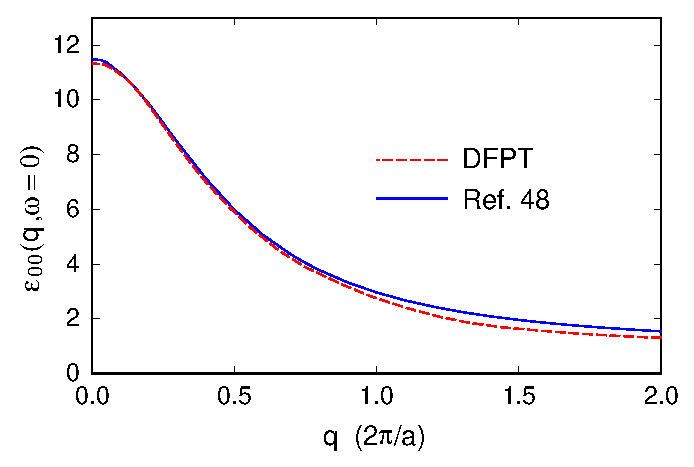
\includegraphics[width=7.5cm]{fig1.eps}
\end    {center}
\caption{\label{fig.pade}
        Comparison of the dielectric function calculated for silicon 
        on the real axis and the analytically continued function starting
        from imaginary frequencies. The three panels correspond to the
        cases illustrated in Fig.\ 3 of Ref.\ \onlinecite{hl86}.
        }
\end    {figure}

\section{Simultaneous calculation of the susceptibility at multiple frequencies}

The linear system given by Eq.\ (\ref{eq.linsys.1}) 
can also be solved efficiently by using a ``multishift'' 
{\tt cBiCG} method.\cite{frommer} 
Multishift methods exploit the knowledge gained during the iterative
solution of the ``seed'' system $Ax=b$ in order to determine the solutions 
of the ``shifted'' system $Ax+\w x=b$, without adding to the the computational 
cost. The logic behind such method is that the seed system and the
shifted system share the same Krilov subspaces $\{b,Ab,A^2b,\cdots\}$,
therefore the residuals of the seed and of the shifted
systems can be taken to be collinear.\cite{frommer}

In practice we can determine the
full frequency-dependent susceptibility 
by performing one single static calculation for each $\q$, $\G$, and $\Gp$.
For the seed system the algorithm is still given by Eqs.\ (\ref{eq.cg1})-(\ref{eq.cg7}).
For the shifted system we replace the calculation of the residuals
$r_{n,\w}$ and of the coefficients $\alpha_{n,\w}$, $\beta_{n,\w}$ by the following relations:
  \begin{equation} \label{eq.shift.1}
  r_{n,\w}  =\frac{r_n}{\pi_{n,\w}};
  \hspace{0.2cm}
  \alpha_{n,\w}  =  \frac{\pi_{n,\w}}{\pi_{n+1,\w}}\alpha_n ;
  \hspace{0.2cm}
  \beta_{n,\w}  =  \Big(\frac{\pi_{n,\w}}{\pi_{n+1,\w}}\Big)^2\beta_n,
  \end{equation}
where the scaling factor $\pi_{n+1,\w}$ is calculated through the recurrence relation
  \begin{equation}\label{eq.shift.2}
  \pi_{n+1,\w} = (1+\w\alpha_n) \pi_{n,\w} + \frac{\alpha_n\beta_{n-1}}{\alpha_{n-1}}(\pi_{n,\w}-\pi_{n-1,\w}).
  \end{equation}
In order to guarantee the collinearity of the residuals, the method
is initialized with $x_0=0$.
The use of Eqs.~(\ref{eq.shift.1}) and (\ref{eq.shift.2}) allows us to
skip the time-consuming operations involving the Hamiltonian in
Eqs.\ (\ref{eq.cg1}) and~(\ref{eq.cg5}).
This method is extremely convienient for determining the frequency-dependent
susceptibility for many frequencies at the cost of one single frequency calculation.
Nevertheless the method presents some practical limitations.

The first major limitation is that the rhs $b$ of the linear system $Ax+\w x=b$
must be the same for all the frequencies considered. In our case
the rhs corresponds to the self-consistent screened perturbation, 
and does depend on the frequency. Therefore if we want to use the
shifted {\tt cBiCG} method we also need to abandon the idea of 
calculating self-consistently the screened Coulomb interaction. 
Instead, we would need to replace this 
by the non-selfconsistent calculation of the susceptibility, followed 
by the explicit inversion of the dielectric matrix for each frequency.
The resulting method constitutes an improved version of the technique
already proposed in Ref.\ \onlinecite{reining}.

The second important limitation is that the shifted {\tt cBiCG} methods
does not allow for the use of effective preconditioners. In fact,
after preconditioning the seed system $M^{-1}Ax=M^{-1}b$ and the shifted
system $M^{-1}Ax+\w M^{-1}x=M^{-1}b$ no longer share the same Krilov subspaces, 
hence the residuals are no longer collinear.\cite{simoncini} 
The practical consequence is that for systems with
large basis set energy cutoffs and small band gaps, the number of iterations
required to achieve convergence can be extremely large.
In addition, the convergence rate of the shifted method is dictated
by the worst-conditioned system, therefore also in this case
we need to perform calculations along the imaginary axis and then anaytically
continue the function to real frequencies.

If we consider that we need approximately 10 frequency points for the
Pad\'e approximants, and each preconditioned calculation requires
in average approximately 10 iterations and 5 self-consistency cycles, 
we conclude that the direct calculation of the screened Coulomb interaction
will be convenient as long as the (non-preconditioned)
shifted {\tt cBiCG} method requires more than $10\times10\times5=500$ 
iterations (assuming that the cost of matrix inversion is negligible).
On the other hand, if we need an ultra-fine sampling of the frequency
dependence, then the shifted method would prove advantageous.

\begin{thebibliography}{99}

\bibitem{hl}
L. Hedin and S. Lundqvist,
Effects of the electron-electron and the electron-phonon interaction in
the one-electron states of solids,
in {\it Solid State Physics}, ed. by F. Seitz, D. Turnbull, and
H. Ehrenreich, (Academic, New York, 1969), vol.\ 23, pag. 1.

\bibitem{hl86}
M. Hybertsen and S. G. Louie, 
Phys.\ Rev.\ B {\bf 34}, 5390 (1986).

\bibitem{painless.cg}
G.\ H.\ Golub and C.\ F.\ Van Loan, {\it Matrix Computations} (John Hopkins University Press, Baltimore, 1983).

\bibitem{jacobs}
D.\ A.\ H.\ Jacobs,
IMA J.\ Numer.\ Anal.\ {\bf 6}, 446 (1986).

\bibitem{baroni.rmp}
S. Baroni, S. de Gironcoli, A. Dal Corso, and P. Giannozi, 
Rev.\ Mod.\ Phys.\ {\bf 73}, 515 (2001).

\bibitem{tpa}
M. P. Teter, M. C. Payne, and D. C. Allan,
Phys.\ Rev.\ B {\bf 40}, 12255 (1989).

\bibitem{pade1}
K.-H. Lee and K. J. Chang,
Phys.\ Rev.\ B {\bf 54}, R8285 (1996).

\bibitem{pade2}
H. J. Vidberg and J. W. Serene,
J.\ Low.\ Temp.\ Phys.\ {\bf 29}, 179 (1977).

\bibitem{pade3}
S. Leb\`egue, B. Arnaud, M. Alouani, and P. E. Bloechl,
Phys.\ Rev.\ B {\bf 67}, 155208 (2003).

\bibitem{godby1}
H. N. Rojas, R. W. Godby, and R. J. Needs,
Phys.\ Rev.\ Lett.\ {\bf 10}, 1827 (1995).

\bibitem{nelder-mead}
J. A. Nelder and R. Mead, 
Comput. J. {\bf 7}, 308 (1965).
We used the implementation available from the
{\tt E04CCF} routine of the {\tt NAG} library
({\tt www.nag.co.uk}).

\bibitem{frommer}
A. Frommer,
Computing {\bf 70}, 87 (2003).

\bibitem{reining}
L. Reining, G. Onida, and R. W. Godby, 
Phys.\ Rev.\ B {\bf 56} R4301 (1997).

\bibitem{simoncini}
V. Simoncini and D. B. Szyld,
Numer.\ Linear Algebr.\ {\bf 14}, 1 (2006).

\bibitem{note.w.even}
Note that from Eq.\ (\ref{eq.p}) it follows that $P(\r,\rp;-\w^\star)=P^\star(\r,\rp;\w)$,
therefore using twice Eq.\ (\ref{eq.w}) (once for $w$ and once for $-w^\star$ and taking
the cc) we obtain $W(\r,\rp;-\w^\star)=W^\star(\r,\rp;\w)$. In other words
the screened interaction is even w.r.t. the imaginary axis.
In particular, in the special case when $\w$ is purely imaginary:
  \begin{equation}
  \Delta n_{[\r,\w]} = 4 {\rm Re} \sum_v \psi_v^\star \Delta \psi_{v[\r,\w]},
  \end{equation}
and we need to solve only one linear systemi because $-\w^\star=\w$,
as in the static case (The factor 4 is for twice the real part times the spin degeneracy).
Note also that for imaginary frequencies the screened interaction is purely real
(in $\r$ space), therefore we need to compute the parturbation for half of the $\G$ vectors in
the small grid (factor 2 speedup).

\bibitem{note.imag1}
In particular, in case of purely imginary frequency we have 
$\Delta n_{[-\G,\w]}=\Delta n^\star{[\G,\w]}$ and $\Delta V_{[-\G,\w]}=\Delta V^\star_{[\G,\w]}$
(reality).


\bibitem{note.grep.1}
  \begin{equation}
  \Delta V^{\rm H}_{[\G,\w]}(\rp) = \int d\rpp \Delta n_{[\G,\w]}(\rpp) \, v(\rpp,\rp),
  \end{equation}
and the screened interaction reads finally:
  \begin{equation}
  \Delta V_{[\G,\w]}(\rp) = v_{[\G]}(\rp) + \Delta V^{\rm H}_{[\G\w]}(\rp).
  \end{equation}

\end{thebibliography}

\end{document}
